\chapter{Линии и графы}

\setlength{\epigraphwidth}{.83\textwidth}
\epigraph{Человеческому сердцу приятен небольшой беспорядок в своей геометрии. ???}{--- Луи де Берниер (1954---)}

%Louis de Bernieres (2012). “Corelli's Mandolin: A Novel”, p.256, Vintage 

Мы спускаемся в одномерный мир --- к кривым, о которых вы знаете, и графам, о которых, возможно, не знаете.
Граф это просто набор точек, называемых вершинами, некоторые пары из которых образуют рёбра.
Часто вершины графа изображаются точками на плоскости, а его рёбра отрезками или кривыми, соединяющими одну свою вершину с другой.
При этом, если возможно обойтись пересечений рёбер друг с другом, то граф называется \emph{планарным}.

\subsection*{Укрепление сетки}

У нас есть сетка размером $n \times n$ из стержней единичной длины, шарнирно соединённых в концах.
Вы можете укрепить некоторый набор $S$ маленьких квадратов диагональными скобками (длиной $\sqrt{2}$).

Какие наборы $S$ достаточны, чтобы сделать сетку жёсткой в плоскости?

\begin{figure}[ht!]
\centering
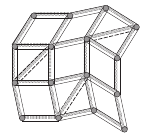
\includegraphics[scale=1]{pics/lattice1}
\caption{Недоукреплённая сетка.}
\label{pic:lattice1}
\end{figure}

На рис. \ref{pic:lattice1} показана (кажущаяся) недостаточно укреплённая сетка размером $3 \times 3$.

\subsection*{Путешествие по острову}

Алоизий катается по острову на своём прекрасном автомобиле.
На каждом перекрёстке острова сходится ровно три (двусторонние) улицы.
Алоизий придерживается следующего правила:
начав с произвольного направления начального перекрёстка, он поворачивает направо на следующем перекрёстке, затем налево на следующем, затем направо, затем налево и так далее.

Докажите, что рано или поздно Алоизий вернётся на перекрёсток, с которого начал.

\parit{Замечание:} Граф, в котором к каждой вершине подходят три ребра, называется \emph{кубическим}.
В нашем графе есть понятия \emph{право} или \emph{лево},
для этого достаточно чтобы граф был изображён на плоскости, с рёбрами (улицами) образованы кривыми.
При этом не обязательно требовать, чтобы граф был планарным;
можно разрешить мосты и туннели, то есть места, где ребра проходят один над другим.

\subsection*{Провода под Гудзоном}

Пятьдесят одинаковых проводов проходят под рекой Гудзон, все они выглядят одинаково.
Требуется определить все пары концов, принадлежащих одному проводу.
Для этого можно замыкать любые проводов вместе на западном конце туннеля и проверять пары концов проводов на восточном конце, чтобы увидеть, образуют ли они замкнутую цепь;
другими словами, вы можете определить, замкнута ли данная пара проводов на другой стороне реки.

Сколько потребуется поездок через Гудзон, чтобы выполнить эту задачу?

\subsection*{Жуки на четырёх прямых}

Даны четыре прямые на плоскости в общем положении (никакие две параллельны, и никакие три не пересекаются в одной точке).
На каждой прямой жук-призрак ползёт с постоянной скоростью (возможно, разной для каждого жука).
Будучи призраками, при встрече жуки продолжают ползти сквозь друг друга.

Докажите, что если было пять из всех шести возможных встреч,
то была и шестая.

\medskip

Ну раз уж мы начали про жуков...

\subsection*{Пауки на кубе}

Три паука и муравей бегают по рёбрам куба.
Каждый паук бегает в три раза медленней муравья.
Докажите, что пауки смогут поймать муравья.

\medskip

Следующая головоломка приводит нас к прекрасной общей теореме графовой теории.

\subsection*{Вменяемые мыслители}

Жители Флоптауна каждую неделю встречаются, чтобы обсуждать городскую политику, в частности, поддерживать ли строительство нового торгового центра в центре города.
Во время встреч каждый гражданин обсуждает этот вопрос со своими друзьями --- по какой-то причине их всегда нечётное число --- и на следующий день, при необходимости, изменяет своё мнение относительно торгового центра так, чтобы оно соответствовало мнению большинства его друзей.

Докажите, что с какого-то момента, каждую вторую неделю у каждого будет то же самое мнение.

\parit{Замечание:}
Поскольку существует только конечное число наборов мнений ($2^n$, если в городе $n$ граждан), очевидно, что рано или поздно произойдёт зацикливание.
В данном случае утверждается, что период цикла должен быть $2$ (или $1$).
Почему такое может быть правдой?

\medskip

И под конец о том, кто хочет остаться на своём графе.

\subsection*{Лемминг на шахматной доске}

На каждой клетке шахматной доски размера $n\times n$ есть стрелка, указывающая на одну из его восьми соседних клеток (или за пределы доски, если это крайняя клетка).
Однако направления стрелок в соседних клетках (включая диагональные) не могут различаться более чем на 45 градусов.

Лемминг начинает свой путь в центральном квадрате, следуя по стрелкам из квадрата в квадрат.
Придётся ли ему непременно упасть с доски?
